\newpage
\chapter{Literature Review}

\textsl{The purpose of the current chapter is to provide knowledge of the subject areas relevant to the project including current developments, controversies, breakthrough, previous research and relevant background theory.}


\section{Market Research Platform}
 

The purpose of the project is to develop a general purpose Market Research Platform that employs big data analytics to produce marketing information and useful insights that small and medium companies can use to understand their market and be more competitive. Marketing research is useful in the area of product planning and development such as when evaluating the need for a new product or its positioning in the market. It has applications in the area of advertising and copy testing or to identify existing and potential distribution channels. It can help to deduce the pricing expectations of consumers and their reactions and responses to different price levels of products. Marketing research can identify the forces operating in a market and assess the market trends, the size of present and potential markets of the company, the evolution of the impact of government legislation, policies, and schemes on the performances of marketing operations of the company. It can also study the sales potential of the company’s products and the evolution of the company’s sales performance. Finally, it can assess the environmental fitness of the firm. \cite{marketingresearch}. A study conducted by the Alibaba Group in China has also shown a way of calculating the impact of brands on society, by combining the impact brands have on the media, the government Impact and the personal impact. \cite{brandsimpact} The marketing platform can obtain all these analytics by integrating several data sources and where necessary apply AI and Machine learning to deduce complex results \cite{marketingml}. Currently, there is no one platform that provides such a varied and unified view of the markets of a business. Platforms like QuantCloud, a trading service \cite{quantcloud}, or Google Analytics, a websites activity tracking platform \cite{googleanalytics}, all offer insights within specific areas and require specialized knowledge to be used. The goal is to build a product that does not require specialized knowledge and that is able to provide as much information as possible. 

\section{Data Extraction, Integration and Processing and Storage}
Data usually comes from a very different a pool of sources such as social media, web server logs, sensors, the stock market, e-mails, etc. and it is no easy task to gather and integrate it all efficiently on a common model. The main challenges of data integration are how to integrate structured and unstructured data, how to manage it and sync it across many data sources. One of the best ways to performs this task is using the Extract, Transform and Load pattern (ETL) \cite{feasibility}. The data is collected from multiple types of sources, mapped to a mutual model and finally stored to a data repository. This process can be made very efficient using a framework such as Spark \cite{spark}.



\newpage
\section{AI, ML and Big Data}
Big data is a term used to describe the huge amount of data that is being generated by organizations in today’s business environment. Such data usually comes from three primary sources: social data such as likes, tweets, comments, video uploads, queries in search engines etc., machine data generated by sensors installed in industrial equipment and transaction data. Machine learning is a branch of artificial intelligence that provides tools and techniques for working on all this data to produce useful results. It based on the idea that systems can learn from data, identify patterns and make decisions with minimal human intervention. Machine learning algorithms are classified into supervised learning, unsupervised learning and reinforcement learning \cite{marketingml}: 
 
\subsection{Supervised learning}

Supervised learning is the task of training a function with labelled training data in order for this function to be able to learn a general rule and map any input to its appropriate output. Machine learning models are usually very good at performing regression and classification:

\begin{itemize} 
\item Statistical modelling techniques are used to find a parametric function that best fits a set of observations and train it appropriately so that is can predict new observations. Statistical models (i.e. logistic models, polynomials, linear regression models) are very good at modelling and predicting trends;
\item Neural networks are powerful tools used to perform regression and classification of non linearly separable data. For example, convolutional neural networks can be used to classify consumers according to their preferences so that they can be targeted by specific ads or marketing strategies \cite{socialtrends}. Neural Networks, paired with Locality sensitive hashing \cite{lsh} have been also used to improve de-duplication, that is to identify chunks that are already stored in a large database;
\item Support Vector Machines are excellent regression and classification algorithms that work by separating data by a hyperplane and maximizing the margin between the closest points. They can be employed to classify social media data such as tweets, posts, comments etc. according to the emotions they emit (positive, negative and neutral). These results can aid in understanding if people have a good or bad opinion about something and take action accordingly \cite{sentimentanalysis}.
\end{itemize}  


\subsection{Unsupervised learning}
Unsupervised learning is a machine learning technique in which a model works on its own to discover hidden patterns and separate unlabelled information into appropriate clusters, if they exist. It is useful for finding associations between different parameters in the available data, for example people that buy X might also buy Y. It can also be used to find the anomalous elements in a data set \cite{kmeans}. There are several clustering methods:
\begin{itemize} 
\item Hierarchical clustering is a naive clustering method that builds a hierarchy of clusters by iteratively joining together the closest elements;
\item K-means is a set of unsupervised clustering algorithms that can divide data points into k clusters  \cite{kmeans};
\item K-Nearest Neighbors is an algorithm that finds the k nearest points to the point of interest.
\end{itemize}

\subsection{Reinforcement learning}
Reinforcement learning is the training of machine learning models to make a sequence of decisions. The agent learns to achieve a goal in an uncertain, potentially complex environment. \cite{reinforcementlearning} Some relevant reinforcement learning algorithms are:
\begin{itemize} 
\item Monte Carlo methods are a way of obtaining estimates when working with uncertain phenomena. They use randomness to obtain meaningful information and are effective for calculating business risks and predicting costs or scheduling overruns;
\item For any finite Markov decision process, Q-learning algorithms are able to find an optimal path by maximizing the expected value of the total reward over any and all successive steps, starting from a specific state. These algorithms can be used to make decisions in business environments, for example in order to determine whether to hold, buy, or sell at any point in time.
\end{itemize}


\section{ML workflow}

\begin{figure}[H]
	\centering
	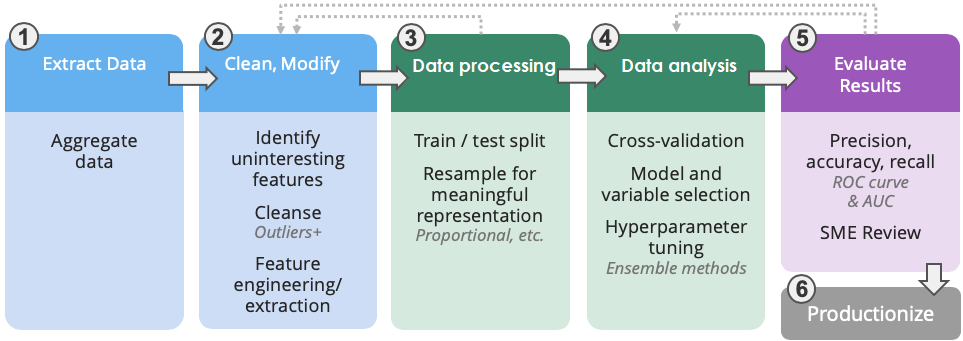
\includegraphics[scale=0.8]{img/mlworkflow.png}
	\caption{ML workflow}
\end{figure} 

A machine learning task typically follows a cycle similar to the diagram above \cite{mlworkflow} and includes data gathering/extraction, data cleaning, data processing, data analysis, training and testing and finally the evaluation phase.


\subsection{Data aggregation}
Data aggregation is the process of gathering data and presenting it in a summarized format. The data may be gathered from multiple data sources with the intent of combining these data sources into a common format.

\subsection{Data cleaning}
Before data can be fed to a training algorithm or used for numerical analysis, it is important to prepare it by removing or changing rows that are incorrect, incomplete, irrelevant, duplicated, or improperly formatted. Skipping this step is not recommended because it can lead to runtime errors, inaccurate results and false conclusions \cite{quantcloud}. 

\subsection{Data processing}
The data is divided into 3 three different sets, the training set, the validation set and the test set. During this phase some dimensions of the data might be removed, merged together or reshaped depending on the kind of task to be performed.

\subsection{Data analysis}
Depending on the task at hand (regression or classification) an array of ML models and sets of optimal hyperparameters are chosen for training. 

\subsection{Evaluation}
The chosen models are trained with the training data and their precision, accuracy and recall are compared in order to find the best model and understand how well the chosen model can work in the future.

\newpage
\section{Tools and Techniques}

There are many tools and technologies that have been  developed for data extraction, integration, processing and analysis. The following tools and techniques have several features that are useful for Big Data integration and Machine learning tasks.

\subsection{Aurelia}
Aurelia is a client-side JavaScript framework that implements the Model-View-View-Model (MVVM) pattern and supports ES6 and TypeScript. It has a very good performance, an extensive ecosystem, it has a very solid and intuitive routing system and employs reactive binding. In Aurelia the presentation layer is completely separated from the application logic and as a result Aurelia applications are very maintainable, testable and extensible. 

\subsection{Django}

\begin{figure}[H]
	\centering
	
\includegraphics[scale=0.15]{img/django.png}
	\caption{Django}
\end{figure} 


Django is a Python framework \cite{django} and is used to write web applications. It comes with a lot of useful APIs, such as an Object relational mapping API, an User authentication module, a HTTP Session handling module etc. The framework employs the Model Template View pattern (MTV), which is a variation of the Model View Controller (MVC). In Django the Model components represent the data and the model classes are mapped automatically to database tables. The View components handle the HTTP requests and return responses. The templates are used to serve the HTML or data for the websites.



\subsection{Spark}

\begin{figure}[H]
	\centering
	
\includegraphics[scale=0.1]{img/spark.png}
	\caption{Spark}
\end{figure} 


Spark is a framework developed in 2009 at UC Berkeley \cite{spark} that provides primitives for data mining and offers a very good implementation of MapReduce, a programming model for processing and generating big data sets with a parallel, distributed algorithm on a cluster \cite{mapreduce}. In Spark every object is a Resilient Distributed Dataset (RDD). The elements of an RDD are not stored in memory but rather every RDDs maintains lineage information for fetching data sets from their source when needed. RDDs can be computed from a HDFS Hadoop Distributed File System (HDFS) or from an existing RDD. In Spark data is split among the different workers by a main driver. Every worker performs its assigned task and then sends the result back to the origin. Spark is up to 100 times faster than Hadoop, because the latter only processes data on disk, while Spark can also load data in memory. As a result, Spark can read 1 TB of data in 4 or 7 seconds. Spark can run on clusters created using many different technologies, such as Apache Mesos, Kubernetes, Amazon EMR etc. and a Spark cluster can scale very easily.

\subsection{Docker}

\begin{figure}[H]
	\centering
	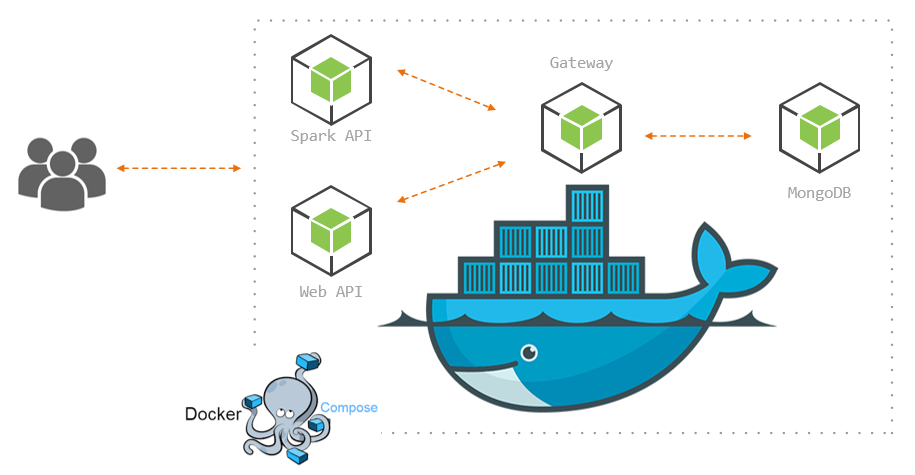
\includegraphics[scale=0.4]{img/docker.png}
	\caption{Docker}
\end{figure}

Docker is a platform for packaging and delivering independent software units in portable and self-sufficient containers that have all the dependencies required for the functionality of their applications. Every container is derived from an image, which essentially is a read-only template. An image provides its container with environmental variables, a command line and a filesystem that can store operating systems, packages, libraries and every other dependency a container needs. The main advantage of encapsulating all the dependencies of a service inside a self-sufficient entity it’s ensuring that the development platform mimics perfectly the target platform. This makes it very easy to continuously integrate and deploy, increases productivity and encourages a frequent feedback loop. With Docker it's possible to package the different types of nodes of an application. \cite{docker}.


\subsection{Query optimization through hashing}
A very good algorithm for optimizing comparison between items is locality sensitive hashing (LSH). LSH uses the properties of hashing in order to find similarities between big sized entities \cite{lsh}.
LSH can be used to improve query efficiency through an approximate Membership Query (AMQ) scheme. In such a system, the items are hashed with a similar process as LSH, with the only difference being that instead of hashing the signature into buckets, a Bloom filter is used in the last step to map every item into L bits. All the items that have the same L bits set to 1 are determined to be approximate members of the same data set S. AMQ can be used to produce results within a search engine in O(1) time and has demonstrated better accuracy than LSB-trees and other algorithms than run in at least logarithmic time. However, a good configuration is needed in order to minimize false positives and false negatives \cite{amq}.








